\section{El problema del viajante de comercio}

\begin{frame}{Problema}
Hallar el recorrido con distancia mínima en un conjunto de
ciudades que pase por todas las ciudades y regrese al punto inicial.

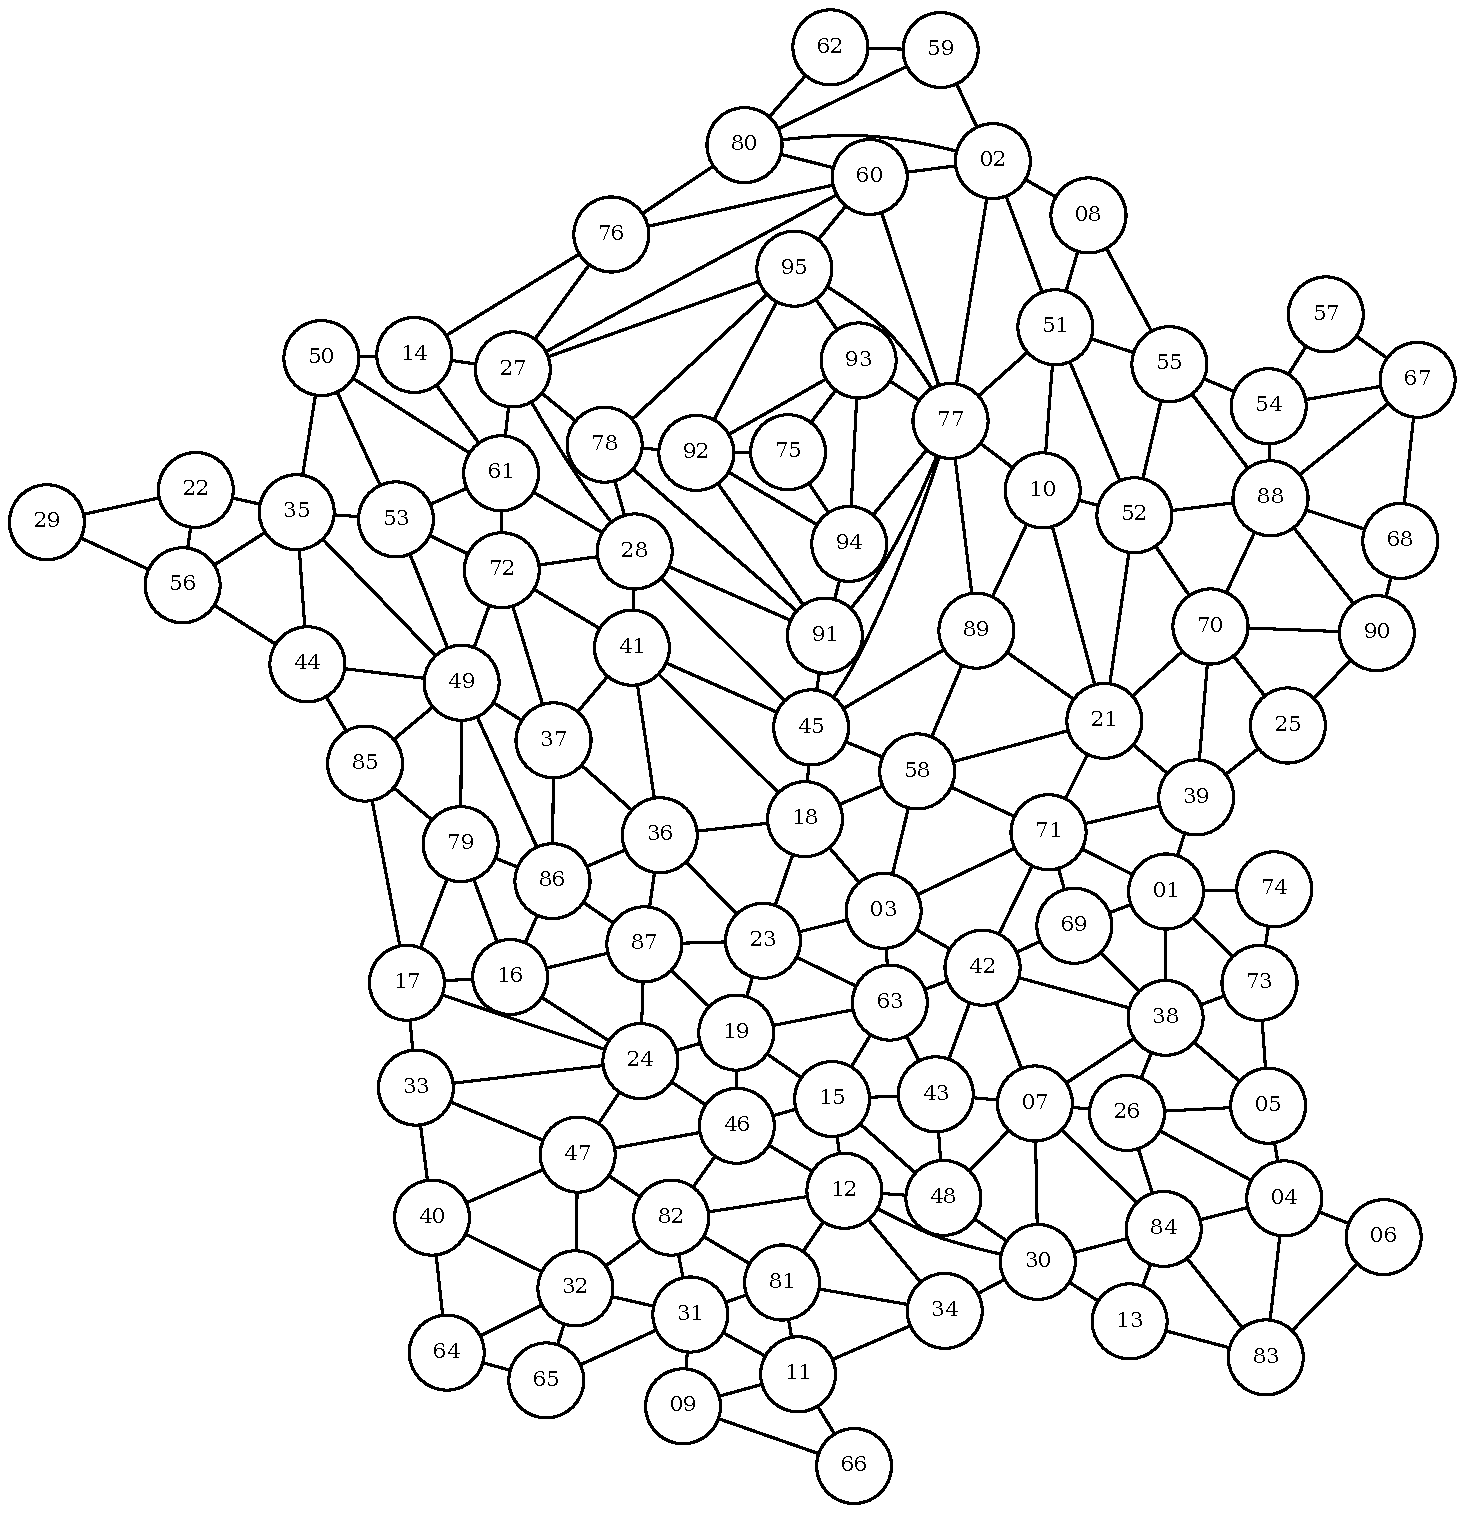
\includegraphics[width=.5\textwidth]{img/Francia} \centering
\end{frame}

\begin{frame}{Algoritmos}
\begin{description}
 \item[Entrada:] Ficheros con ciudades indicadas como puntos en el plano según sus
 coordenadas.
 \item[Salida:] \texttt{vector<int>} con el orden en el que se recorren las ciudades.
\end{description}
\end{frame}

% TODO: todo lo posterior

\begin{frame}{\texttt{Grafo}}
Un grafo consta de:

\begin{itemize}
  \item Una \textbf{cantidad de nodos}: \texttt{nodos}.
  \item Una \textbf{matriz de pesos}: \texttt{lados}.
\end{itemize}
\end{frame}

\section{Ramificación y acotación (Branch and Bound)}

\subsection{Ramificación y acotación}

\begin{frame}{Algoritmo Branch and Bound}
  Iniciamos:
  \begin{itemize}
    \item La cola con prioridad con la solución parcial \texttt{[0]}
    \item La mejor solución con un algoritmo \textit{greedy} (vecino más cercano)
  \end{itemize}
\end{frame}

\begin{frame}{Algoritmo Branch and Bound}
  Mientras la cola no esté vacía y la cota del primer elemento esté por debajo de la mejor solución, coge el primer elemento:
  \begin{itemize}
    \item Si \textbf{puede formarse una solución completa}, comprueba si es mejor que la mejor encontrada. En tal caso se actualiza.
    \item En \textbf{otro caso}, para cada ciudad no visitada forma una nueva solución parcial. Se añade a la cola si su cota es mejor que la mejor solución.
  \end{itemize}
\end{frame}

\section{Cotas (Branch and Bound)}

\begin{frame}{Cota del mínimo}
  Calcular la longitud del recorrido inicial y sumar la menor distancia de cada ciudad no incluida en la solución parcial con sus relacionadas.
\end{frame}

\begin{frame}{Árbol generador}
  Calcular la longitud del recorrido que se lleva hasta ese momento, y sumar la longitud del árbol generador minimal que se forma desde el camino que ya llevamos. Además, se suma la mínima longitud del primer nodo a otro más.

  %% Aquí pintad en pizarra que si no, no lo entiende ni dios, y es una tontería
\end{frame}

\section{Vuelta atrás (Backtracking)}

\subsection{Vuelta atrás}

\begin{frame}{Algoritmo Backtracking}
  Desde un nodo inicial, vamos tomando todas las posibilidades mediante una llamada recursiva. Si al añadir un nodo hace que el camino mida más que nuestro camino más corto hasta el momento, se deja esa posibilidad, y se vuelve atrás.
  
  Aquí no interviene ninguna cota inferior, y se trabaja con la longitud del mejor camino hasta el momento como cota superior.
\end{frame}

\begin{frame}[fragile]{Llamada inicial}
\begin{lstlisting}
vector<int> tsp_backtracking(const Grafo<peso_t>& g) {
	vector<int> primera_solucion = tsp_greedy(g);
	int mejor_longitud = longitud(primera_solucion,g);
	vector<int> inicial = {0};
	vector<int> solucion; // Se modifica

	tsp_back_rec(solucion,inicial,mejor_longitud,g);

	return solucion;
}
\end{lstlisting}
\end{frame}

\section{Comparación de algoritmos}

\subsection{Comparativa}

\begin{frame}{Comparación de caminos óptimos}
	Se han escogido tres ejemplos de grafos (de 5, 10 y 12 nodos), y se comparará el camino óptimo tomado por cada algoritmo en cada caso.
	
	Esto nos hace ver que, siendo la longitud del camino óptimo la misma independientemente del algoritmo, el camino óptimo no tiene por qué ser el mismo.
\end{frame}

\begin{frame}{5 ciudades (BaB cota 1, Backtracking)}
	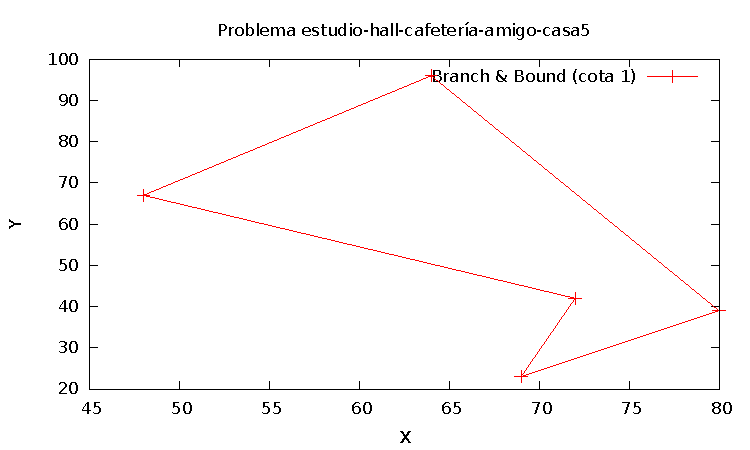
\includegraphics[width=\textwidth]{img/e-h-c-a-c5_tsp_1}
\end{frame}

\begin{frame}{5 ciudades (BaB cota 2)}
	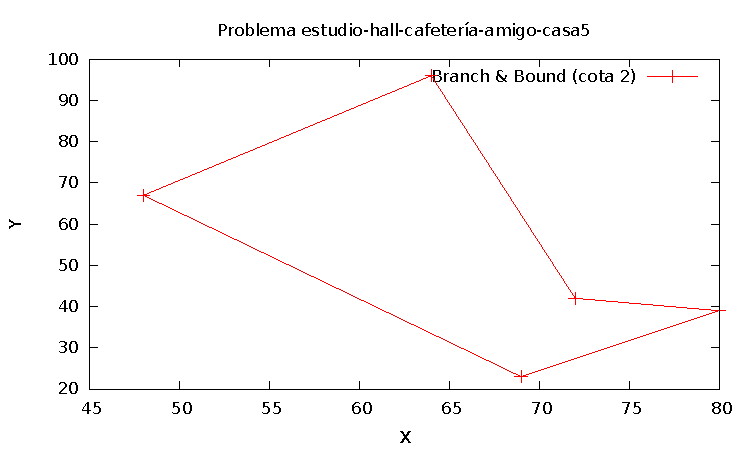
\includegraphics[width=\textwidth]{img/e-h-c-a-c5_tsp_2}
\end{frame}

\begin{frame}{10 ciudades (BaB cota 1)}
	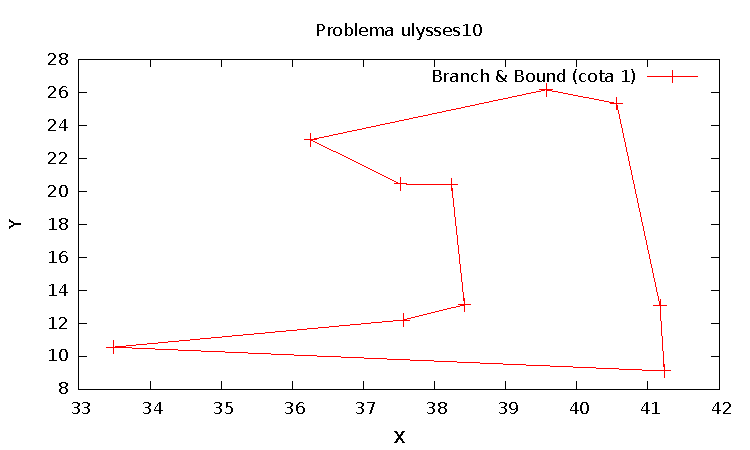
\includegraphics[width=\textwidth]{img/ulysses10_tsp_1}
\end{frame}

\begin{frame}{10 ciudades (BaB cota 2)}
	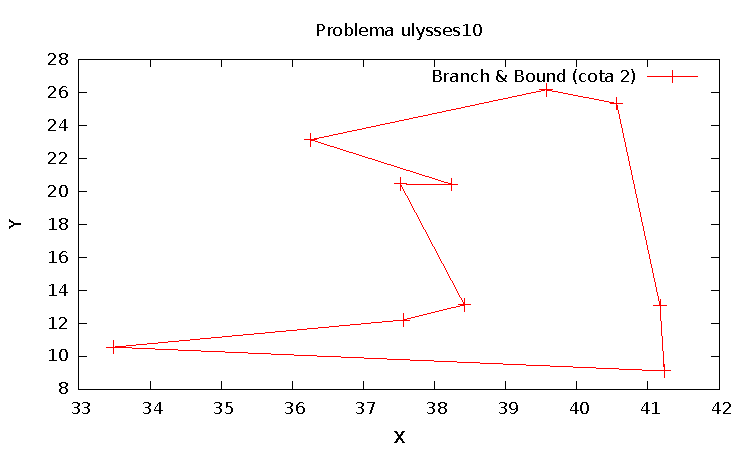
\includegraphics[width=\textwidth]{img/ulysses10_tsp_2}
\end{frame}

\begin{frame}{10 ciudades (Backtracking)}
	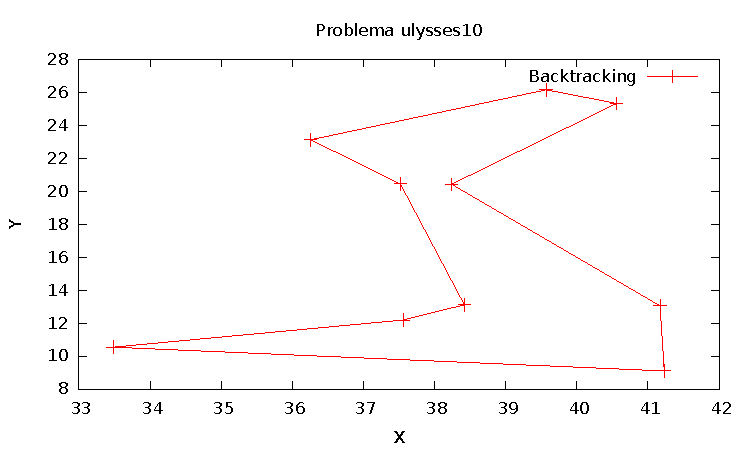
\includegraphics[width=\textwidth]{img/ulysses10_tsp_3}
\end{frame}

\begin{frame}{12 ciudades (Todos)}
	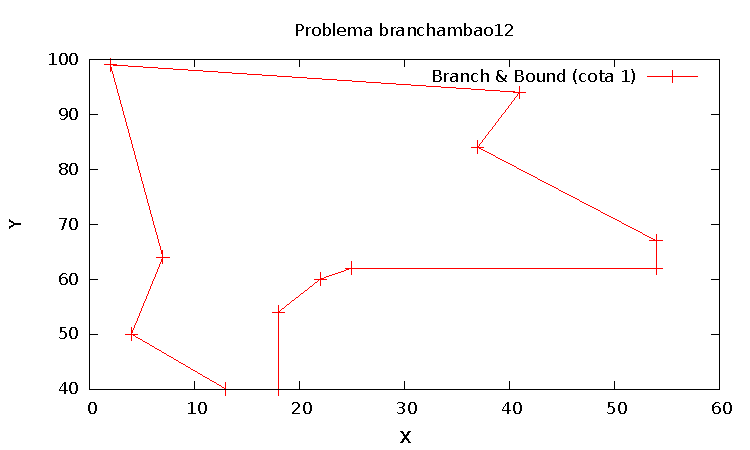
\includegraphics[width=\textwidth]{img/branchambao12_tsp_1}
\end{frame}

\begin{frame}{Comparación de datos}
	Se presenta a continuación la comparación de tiempo, nodos expandidos, podas y tamaño máximo de la cola (en Branch and Bound) en cada uno de los tres ejemplos; grafos de 5, 10 y 12 nodos.
\end{frame}

\begin{frame}{5 ciudades (tiempos)}
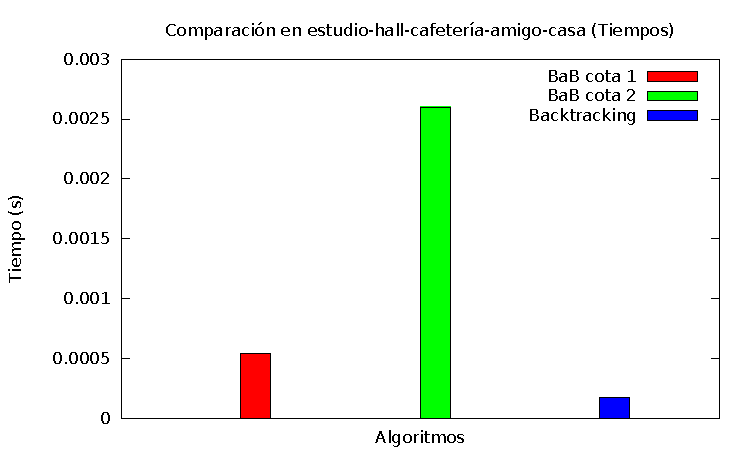
\includegraphics[width=\textwidth]{img/barras_e-h-c-a-c5_t}
\end{frame}

\begin{frame}{5 ciudades (nodos expandidos)}
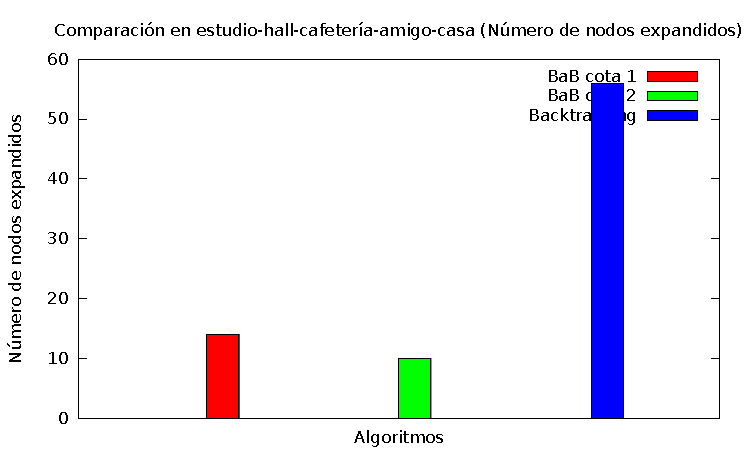
\includegraphics[width=\textwidth]{img/barras_e-h-c-a-c5_nodos}
\end{frame}

\begin{frame}{5 ciudades (podas)}
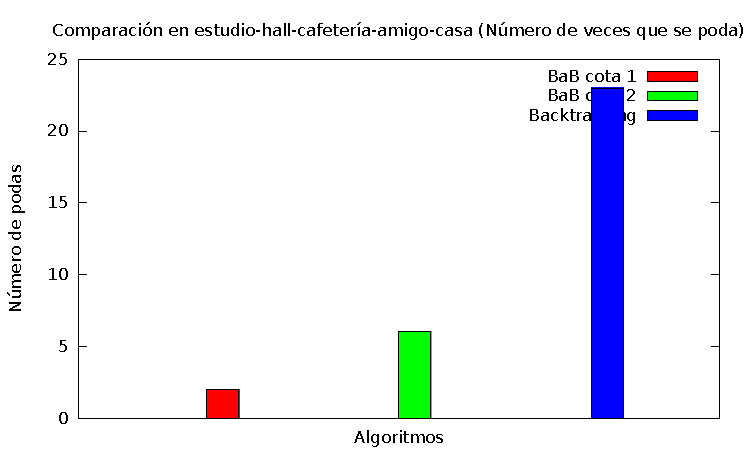
\includegraphics[width=\textwidth]{img/barras_e-h-c-a-c5_poda}
\end{frame}

\begin{frame}{5 ciudades (cola)}
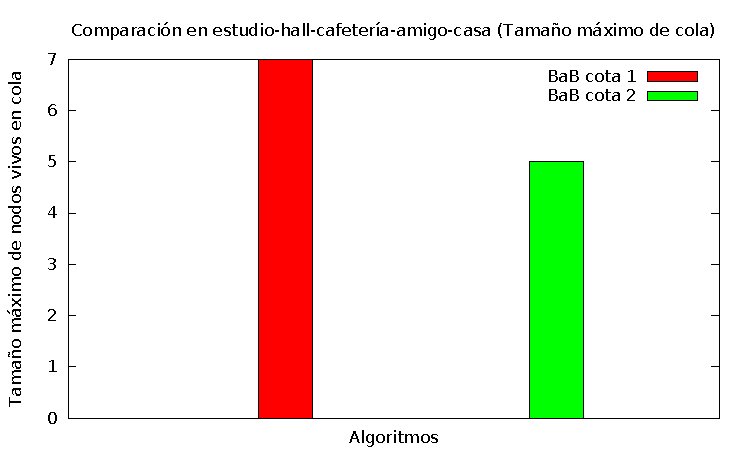
\includegraphics[width=\textwidth]{img/barras_e-h-c-a-c5_cola}
\end{frame}

\begin{frame}{10 ciudades (tiempos)}
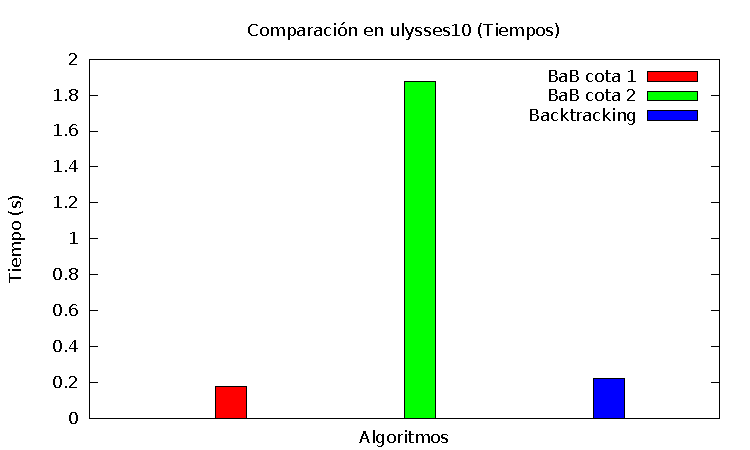
\includegraphics[width=\textwidth]{img/barras_ulysses10_t}
\end{frame}

\begin{frame}{10 ciudades (nodos expandidos)}
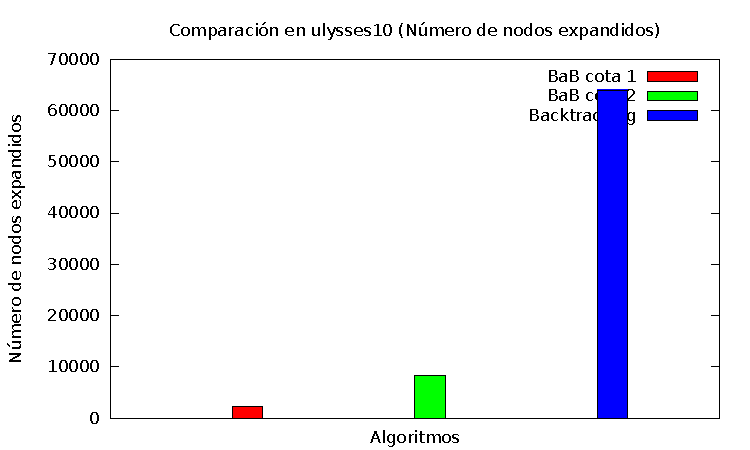
\includegraphics[width=\textwidth]{img/barras_ulysses10_nodos}
\end{frame}

\begin{frame}{10 ciudades (podas)}
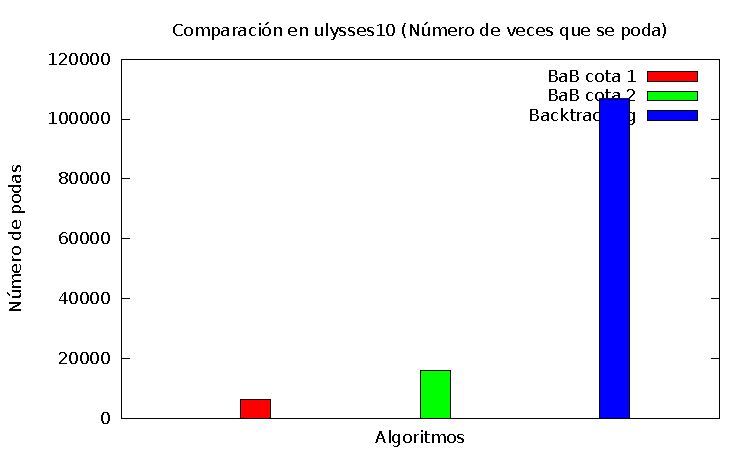
\includegraphics[width=\textwidth]{img/barras_ulysses10_poda}
\end{frame}

\begin{frame}{10 ciudades (cola)}
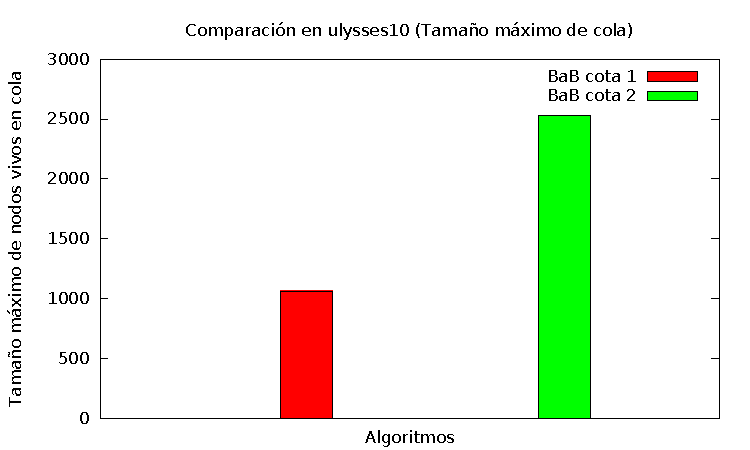
\includegraphics[width=\textwidth]{img/barras_ulysses10_cola}
\end{frame}

\begin{frame}{12 ciudades (tiempos)}
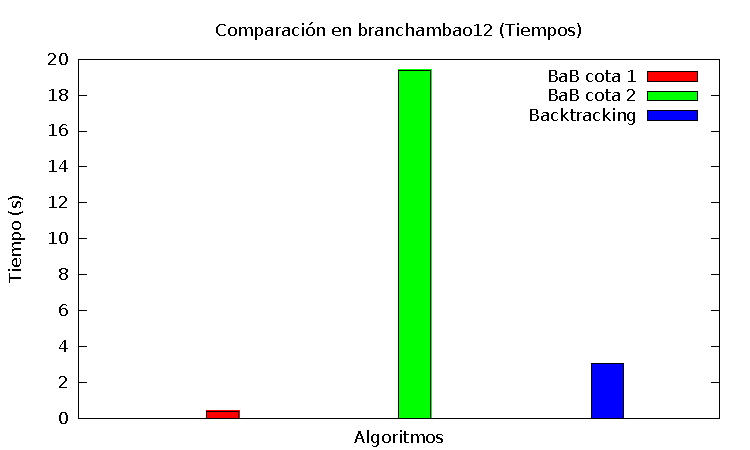
\includegraphics[width=\textwidth]{img/barras_branchambao12_t}
\end{frame}

\begin{frame}{12 ciudades (nodos expandidos)}
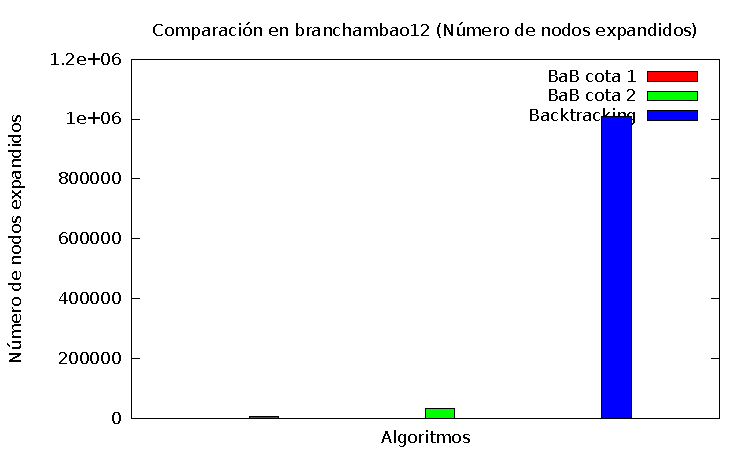
\includegraphics[width=\textwidth]{img/barras_branchambao12_nodos}
\end{frame}

\begin{frame}{12 ciudades (podas)}
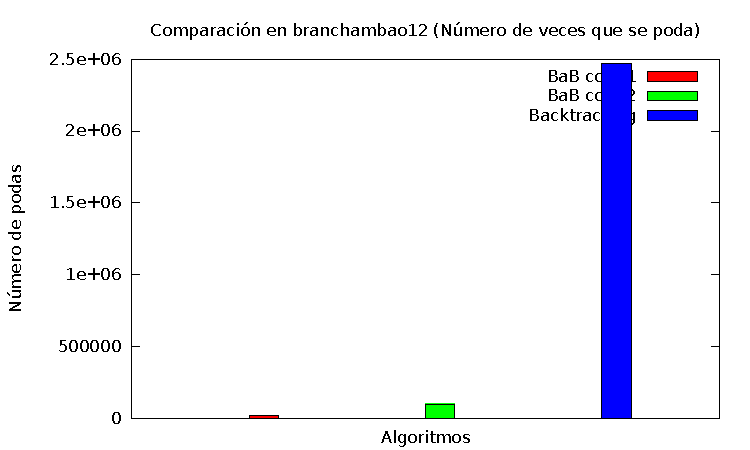
\includegraphics[width=\textwidth]{img/barras_branchambao12_poda}
\end{frame}

\begin{frame}{12 ciudades (cola)}
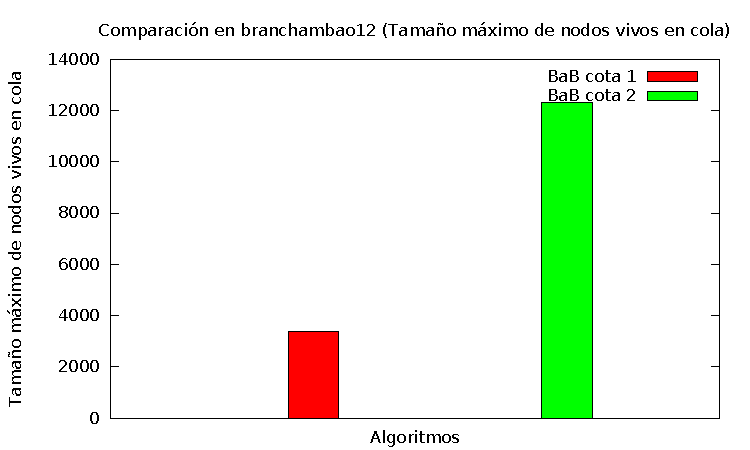
\includegraphics[width=\textwidth]{img/barras_branchambao12_cola}
\end{frame}
